%% bare_conf_compsoc.tex
%% V1.4b
%% 2015/08/26
%% by Michael Shell
%% See:
%% http://www.michaelshell.org/
%% for current contact information.
%%
%% This is a skeleton file demonstrating the use of IEEEtran.cls
%% (requires IEEEtran.cls version 1.8b or later) with an IEEE Computer
%% Society conference paper.
%%
%% Support sites:
%% http://www.michaelshell.org/tex/ieeetran/
%% http://www.ctan.org/pkg/ieeetran
%% and
%% http://www.ieee.org/

%%*************************************************************************
%% Legal Notice:
%% This code is offered as-is without any warranty either expressed or
%% implied; without even the implied warranty of MERCHANTABILITY or
%% FITNESS FOR A PARTICULAR PURPOSE! 
%% User assumes all risk.
%% In no event shall the IEEE or any contributor to this code be liable for
%% any damages or losses, including, but not limited to, incidental,
%% consequential, or any other damages, resulting from the use or misuse
%% of any information contained here.
%%
%% All comments are the opinions of their respective authors and are not
%% necessarily endorsed by the IEEE.
%%
%% This work is distributed under the LaTeX Project Public License (LPPL)
%% ( http://www.latex-project.org/ ) version 1.3, and may be freely used,
%% distributed and modified. A copy of the LPPL, version 1.3, is included
%% in the base LaTeX documentation of all distributions of LaTeX released
%% 2003/12/01 or later.
%% Retain all contribution notices and credits.
%% ** Modified files should be clearly indicated as such, including  **
%% ** renaming them and changing author support contact information. **
%%*************************************************************************


% *** Authors should verify (and, if needed, correct) their LaTeX system  ***
% *** with the testflow diagnostic prior to trusting their LaTeX platform ***
% *** with production work. The IEEE's font choices and paper sizes can   ***
% *** trigger bugs that do not appear when using other class files.       ***                          ***
% The testflow support page is at:
% http://www.michaelshell.org/tex/testflow/



\documentclass[conference,compsoc]{IEEEtran}
% Some/most Computer Society conferences require the compsoc mode option,
% but others may want the standard conference format.
%
% If IEEEtran.cls has not been installed into the LaTeX system files,
% manually specify the path to it like:
% \documentclass[conference,compsoc]{../sty/IEEEtran}





% Some very useful LaTeX packages include:
% (uncomment the ones you want to load)


% *** MISC UTILITY PACKAGES ***
%
%\usepackage{ifpdf}
% Heiko Oberdiek's ifpdf.sty is very useful if you need conditional
% compilation based on whether the output is pdf or dvi.
% usage:
% \ifpdf
%   % pdf code
% \else
%   % dvi code
% \fi
% The latest version of ifpdf.sty can be obtained from:
% http://www.ctan.org/pkg/ifpdf
% Also, note that IEEEtran.cls V1.7 and later provides a builtin
% \ifCLASSINFOpdf conditional that works the same way.
% When switching from latex to pdflatex and vice-versa, the compiler may
% have to be run twice to clear warning/error messages.





\usepackage[hidelinks]{hyperref}
\usepackage{amsmath}
\usepackage{enumerate}
% *** CITATION PACKAGES ***
%
\ifCLASSOPTIONcompsoc
  % IEEE Computer Society needs nocompress option
  % requires cite.sty v4.0 or later (November 2003)
  \usepackage[nocompress]{cite}
\else
  % normal IEEE
  \usepackage{cite}
\fi
% cite.sty was written by Donald Arseneau
% V1.6 and later of IEEEtran pre-defines the format of the cite.sty package
% \cite{} output to follow that of the IEEE. Loading the cite package will
% result in citation numbers being automatically sorted and properly
% "compressed/ranged". e.g., [1], [9], [2], [7], [5], [6] without using
% cite.sty will become [1], [2], [5]--[7], [9] using cite.sty. cite.sty's
% \cite will automatically add leading space, if needed. Use cite.sty's
% noadjust option (cite.sty V3.8 and later) if you want to turn this off
% such as if a citation ever needs to be enclosed in parenthesis.
% cite.sty is already installed on most LaTeX systems. Be sure and use
% version 5.0 (2009-03-20) and later if using hyperref.sty.
% The latest version can be obtained at:
% http://www.ctan.org/pkg/cite
% The documentation is contained in the cite.sty file itself.
%
% Note that some packages require special options to format as the Computer
% Society requires. In particular, Computer Society  papers do not use
% compressed citation ranges as is done in typical IEEE papers
% (e.g., [1]-[4]). Instead, they list every citation separately in order
% (e.g., [1], [2], [3], [4]). To get the latter we need to load the cite
% package with the nocompress option which is supported by cite.sty v4.0
% and later.





% *** GRAPHICS RELATED PACKAGES ***
%
\ifCLASSINFOpdf
  \usepackage[pdftex]{graphicx}
  % declare the path(s) where your graphic files are
  % \graphicspath{{../pdf/}{../jpeg/}}
  % and their extensions so you won't have to specify these with
  % every instance of \includegraphics
  % \DeclareGraphicsExtensions{.pdf,.jpeg,.png}
\else
  % or other class option (dvipsone, dvipdf, if not using dvips). graphicx
  % will default to the driver specified in the system graphics.cfg if no
  % driver is specified.
  % \usepackage[dvips]{graphicx}
  % declare the path(s) where your graphic files are
  % \graphicspath{{../eps/}}
  % and their extensions so you won't have to specify these with
  % every instance of \includegraphics
  % \DeclareGraphicsExtensions{.eps}
\fi
% graphicx was written by David Carlisle and Sebastian Rahtz. It is
% required if you want graphics, photos, etc. graphicx.sty is already
% installed on most LaTeX systems. The latest version and documentation
% can be obtained at: 
% http://www.ctan.org/pkg/graphicx
% Another good source of documentation is "Using Imported Graphics in
% LaTeX2e" by Keith Reckdahl which can be found at:
% http://www.ctan.org/pkg/epslatex
%
% latex, and pdflatex in dvi mode, support graphics in encapsulated
% postscript (.eps) format. pdflatex in pdf mode supports graphics
% in .pdf, .jpeg, .png and .mps (metapost) formats. Users should ensure
% that all non-photo figures use a vector format (.eps, .pdf, .mps) and
% not a bitmapped formats (.jpeg, .png). The IEEE frowns on bitmapped formats
% which can result in "jaggedy"/blurry rendering of lines and letters as
% well as large increases in file sizes.
%
% You can find documentation about the pdfTeX application at:
% http://www.tug.org/applications/pdftex





% *** MATH PACKAGES ***
%
%\usepackage{amsmath}
% A popular package from the American Mathematical Society that provides
% many useful and powerful commands for dealing with mathematics.
%
% Note that the amsmath package sets \interdisplaylinepenalty to 10000
% thus preventing page breaks from occurring within multiline equations. Use:
%\interdisplaylinepenalty=2500
% after loading amsmath to restore such page breaks as IEEEtran.cls normally
% does. amsmath.sty is already installed on most LaTeX systems. The latest
% version and documentation can be obtained at:
% http://www.ctan.org/pkg/amsmath





% *** SPECIALIZED LIST PACKAGES ***
%
\usepackage{algorithmic}
% algorithmic.sty was written by Peter Williams and Rogerio Brito.
% This package provides an algorithmic environment fo describing algorithms.
% You can use the algorithmic environment in-text or within a figure
% environment to provide for a floating algorithm. Do NOT use the algorithm
% floating environment provided by algorithm.sty (by the same authors) or
% algorithm2e.sty (by Christophe Fiorio) as the IEEE does not use dedicated
% algorithm float types and packages that provide these will not provide
% correct IEEE style captions. The latest version and documentation of
% algorithmic.sty can be obtained at:
% http://www.ctan.org/pkg/algorithms
% Also of interest may be the (relatively newer and more customizable)
% algorithmicx.sty package by Szasz Janos:
% http://www.ctan.org/pkg/algorithmicx




% *** ALIGNMENT PACKAGES ***
%
\usepackage{array}
% Frank Mittelbach's and David Carlisle's array.sty patches and improves
% the standard LaTeX2e array and tabular environments to provide better
% appearance and additional user controls. As the default LaTeX2e table
% generation code is lacking to the point of almost being broken with
% respect to the quality of the end results, all users are strongly
% advised to use an enhanced (at the very least that provided by array.sty)
% set of table tools. array.sty is already installed on most systems. The
% latest version and documentation can be obtained at:
% http://www.ctan.org/pkg/array


% IEEEtran contains the IEEEeqnarray family of commands that can be used to
% generate multiline equations as well as matrices, tables, etc., of high
% quality.




% *** SUBFIGURE PACKAGES ***
%\ifCLASSOPTIONcompsoc
 \usepackage[caption=false,font=footnotesize,labelfont=sf,textfont=sf]{subfig}
%\else
 \usepackage[caption=false,font=footnotesize]{subfig}
%\fi
% subfig.sty, written by Steven Douglas Cochran, is the modern replacement
% for subfigure.sty, the latter of which is no longer maintained and is
% incompatible with some LaTeX packages including fixltx2e. However,
% subfig.sty requires and automatically loads Axel Sommerfeldt's caption.sty
% which will override IEEEtran.cls' handling of captions and this will result
% in non-IEEE style figure/table captions. To prevent this problem, be sure
% and invoke subfig.sty's "caption=false" package option (available since
% subfig.sty version 1.3, 2005/06/28) as this is will preserve IEEEtran.cls
% handling of captions.
% Note that the Computer Society format requires a sans serif font rather
% than the serif font used in traditional IEEE formatting and thus the need
% to invoke different subfig.sty package options depending on whether
% compsoc mode has been enabled.
%
% The latest version and documentation of subfig.sty can be obtained at:
% http://www.ctan.org/pkg/subfig




% *** FLOAT PACKAGES ***
%
%\usepackage{fixltx2e}
% fixltx2e, the successor to the earlier fix2col.sty, was written by
% Frank Mittelbach and David Carlisle. This package corrects a few problems
% in the LaTeX2e kernel, the most notable of which is that in current
% LaTeX2e releases, the ordering of single and double column floats is not
% guaranteed to be preserved. Thus, an unpatched LaTeX2e can allow a
% single column figure to be placed prior to an earlier double column
% figure.
% Be aware that LaTeX2e kernels dated 2015 and later have fixltx2e.sty's
% corrections already built into the system in which case a warning will
% be issued if an attempt is made to load fixltx2e.sty as it is no longer
% needed.
% The latest version and documentation can be found at:
% http://www.ctan.org/pkg/fixltx2e


%\usepackage{stfloats}
% stfloats.sty was written by Sigitas Tolusis. This package gives LaTeX2e
% the ability to do double column floats at the bottom of the page as well
% as the top. (e.g., "\begin{figure*}[!b]" is not normally possible in
% LaTeX2e). It also provides a command:
%\fnbelowfloat
% to enable the placement of footnotes below bottom floats (the standard
% LaTeX2e kernel puts them above bottom floats). This is an invasive package
% which rewrites many portions of the LaTeX2e float routines. It may not work
% with other packages that modify the LaTeX2e float routines. The latest
% version and documentation can be obtained at:
% http://www.ctan.org/pkg/stfloats
% Do not use the stfloats baselinefloat ability as the IEEE does not allow
% \baselineskip to stretch. Authors submitting work to the IEEE should note
% that the IEEE rarely uses double column equations and that authors should try
% to avoid such use. Do not be tempted to use the cuted.sty or midfloat.sty
% packages (also by Sigitas Tolusis) as the IEEE does not format its papers in
% such ways.
% Do not attempt to use stfloats with fixltx2e as they are incompatible.
% Instead, use Morten Hogholm'a dblfloatfix which combines the features
% of both fixltx2e and stfloats:
%
% \usepackage{dblfloatfix}
% The latest version can be found at:
% http://www.ctan.org/pkg/dblfloatfix




% *** PDF, URL AND HYPERLINK PACKAGES ***
%
%\usepackage{url}
% url.sty was written by Donald Arseneau. It provides better support for
% handling and breaking URLs. url.sty is already installed on most LaTeX
% systems. The latest version and documentation can be obtained at:
% http://www.ctan.org/pkg/url
% Basically, \url{my_url_here}.




% *** Do not adjust lengths that control margins, column widths, etc. ***
% *** Do not use packages that alter fonts (such as pslatex).         ***
% There should be no need to do such things with IEEEtran.cls V1.6 and later.
% (Unless specifically asked to do so by the journal or conference you plan
% to submit to, of course. )


% correct bad hyphenation here
\hyphenation{op-tical net-works semi-conduc-tor}


\begin{document}
%
% paper title
% Titles are generally capitalized except for words such as a, an, and, as,
% at, but, by, for, in, nor, of, on, or, the, to and up, which are usually
% not capitalized unless they are the first or last word of the title.
% Linebreaks \\ can be used within to get better formatting as desired.
% Do not put math or special symbols in the title.
\title{SFM-MVS to Mesh}


% author names and affiliations
% use a multiple column layout for up to three different
% affiliations
\author{\IEEEauthorblockN{Roderick Lan}
\IEEEauthorblockA{1706751}
\and
\IEEEauthorblockN{Abdullah Khadelli}
\IEEEauthorblockA{1722102}
}

% conference papers do not typically use \thanks and this command
% is locked out in conference mode. If really needed, such as for
% the acknowledgment of grants, issue a \IEEEoverridecommandlockouts
% after \documentclass

% for over three affiliations, or if they all won't fit within the width
% of the page (and note that there is less available width in this regard for
% compsoc conferences compared to traditional conferences), use this
% alternative format:
% 
%\author{\IEEEauthorblockN{Michael Shell\IEEEauthorrefmark{1},
%Homer Simpson\IEEEauthorrefmark{2},
%James Kirk\IEEEauthorrefmark{3}, 
%Montgomery Scott\IEEEauthorrefmark{3} and
%Eldon Tyrell\IEEEauthorrefmark{4}}
%\IEEEauthorblockA{\IEEEauthorrefmark{1}School of Electrical and Computer Engineering\\
%Georgia Institute of Technology,
%Atlanta, Georgia 30332--0250\\ Email: see http://www.michaelshell.org/contact.html}
%\IEEEauthorblockA{\IEEEauthorrefmark{2}Twentieth Century Fox, Springfield, USA\\
%Email: homer@thesimpsons.com}
%\IEEEauthorblockA{\IEEEauthorrefmark{3}Starfleet Academy, San Francisco, California 96678-2391\\
%Telephone: (800) 555--1212, Fax: (888) 555--1212}
%\IEEEauthorblockA{\IEEEauthorrefmark{4}Tyrell Inc., 123 Replicant Street, Los Angeles, California 90210--4321}}




% use for special paper notices
%\IEEEspecialpapernotice{(Invited Paper)}




% make the title area
\maketitle

% As a general rule, do not put math, special symbols or citations
% in the abstract
\begin{abstract}
    Structure From Motion (SFM) and Multiview Stereo (MVS) are computer vision
    algorithms commonly found in a wide range of domains and use cases, 
    one of the most prevalent being photogrammetry. In this project, 
    we investigate the ideal methodology and object properties for photogrammetry 
    of specific objects using SFM, and explore an altered approach to the feature 
    extraction and feature matching steps in the algorithm. Additionally, we evaluate 
    the effectiveness of two algorithms for surface reconstruction on our SFM-MVS 
    (point cloud) outputs. 
\end{abstract}

% no keywords




% For peer review papers, you can put extra information on the cover
% page as needed:
% \ifCLASSOPTIONpeerreview
% \begin{center} \bfseries EDICS Category: 3-BBND \end{center}
% \fi
%
% For peerreview papers, this IEEEtran command inserts a page break and
% creates the second title. It will be ignored for other modes.
\IEEEpeerreviewmaketitle



\section{Introduction}
% no \IEEEPARstart
One of the most common applications of Structure From Motion (SFM) 
and Multiview Stereo (MVS) is in photogrammetry. These two techniques 
are complementary to each other, and result in a dense point cloud reconstruction 
of an object (or environment) from image data. However, in many fields where 
photogrammetry is used, a 3D mesh is likely more useful than a point cloud is. 
As such, time is often spent cleaning resultant point clouds and converting them 
to meshes, when the brunt of this process could be automated and simplified. 
Furthermore, SFM can be relatively slow for many datasets. The general outline of 
SFM algorithms involves feature extraction, feature matching, triangulation and 
bundle adjustment. Each of these steps can take considerable time, however there 
is not much to change with regards to triangulation and bundle adjustment. 
On the other hand, feature extraction (SIFT \cite{sift} based) and feature 
matching can be altered to be computationally faster at a minimal 
cost to accuracy. In a nutshell, this project report will explore 
proposed alterations to feature extraction and feature matching in SFM, 
investigate the ideal methodologies and object types for this altered 
approach, and evaluate algorithms relating to point cloud processing and 
mesh reconstruction. The source code for the project can be found on
\href{https://github.com/roddylan/SFM-to-Mesh}{GitHub}.

% \hfill mds
 
% \hfill August 26, 2015

% \subsection{Subsection Heading Here}
% Subsection text here.


% \subsubsection{Subsubsection Heading Here}
% Subsubsection text here.


% An example of a floating figure using the graphicx package.
% Note that \label must occur AFTER (or within) \caption.
% For figures, \caption should occur after the \includegraphics.
% Note that IEEEtran v1.7 and later has special internal code that
% is designed to preserve the operation of \label within \caption
% even when the captionsoff option is in effect. However, because
% of issues like this, it may be the safest practice to put all your
% \label just after \caption rather than within \caption{}.
%
% Reminder: the "draftcls" or "draftclsnofoot", not "draft", class
% option should be used if it is desired that the figures are to be
% displayed while in draft mode.
%
%\begin{figure}[!t]
%\centering
%\includegraphics[width=2.5in]{myfigure}
% where an .eps filename suffix will be assumed under latex, 
% and a .pdf suffix will be assumed for pdflatex; or what has been declared
% via \DeclareGraphicsExtensions.
%\caption{Simulation results for the network.}
%\label{fig_sim}
%\end{figure}

% Note that the IEEE typically puts floats only at the top, even when this
% results in a large percentage of a column being occupied by floats.


% An example of a double column floating figure using two subfigures.
% (The subfig.sty package must be loaded for this to work.)
% The subfigure \label commands are set within each subfloat command,
% and the \label for the overall figure must come after \caption.
% \hfil is used as a separator to get equal spacing.
% Watch out that the combined width of all the subfigures on a 
% line do not exceed the text width or a line break will occur.
%
%\begin{figure*}[!t]
%\centering
%\subfloat[Case I]{\includegraphics[width=2.5in]{box}%
%\label{fig_first_case}}
%\hfil
%\subfloat[Case II]{\includegraphics[width=2.5in]{box}%
%\label{fig_second_case}}
%\caption{Simulation results for the network.}
%\label{fig_sim}
%\end{figure*}
%
% Note that often IEEE papers with subfigures do not employ subfigure
% captions (using the optional argument to \subfloat[]), but instead will
% reference/describe all of them (a), (b), etc., within the main caption.
% Be aware that for subfig.sty to generate the (a), (b), etc., subfigure
% labels, the optional argument to \subfloat must be present. If a
% subcaption is not desired, just leave its contents blank,
% e.g., \subfloat[].


% An example of a floating table. Note that, for IEEE style tables, the
% \caption command should come BEFORE the table and, given that table
% captions serve much like titles, are usually capitalized except for words
% such as a, an, and, as, at, but, by, for, in, nor, of, on, or, the, to
% and up, which are usually not capitalized unless they are the first or
% last word of the caption. Table text will default to \footnotesize as
% the IEEE normally uses this smaller font for tables.
% The \label must come after \caption as always.
%
%\begin{table}[!t]
%% increase table row spacing, adjust to taste
%\renewcommand{\arraystretch}{1.3}
% if using array.sty, it might be a good idea to tweak the value of
% \extrarowheight as needed to properly center the text within the cells
%\caption{An Example of a Table}
%\label{table_example}
%\centering
%% Some packages, such as MDW tools, offer better commands for making tables
%% than the plain LaTeX2e tabular which is used here.
%\begin{tabular}{|c||c|}
%\hline
%One & Two\\
%\hline
%Three & Four\\
%\hline
%\end{tabular}
%\end{table}


% Note that the IEEE does not put floats in the very first column
% - or typically anywhere on the first page for that matter. Also,
% in-text middle ("here") positioning is typically not used, but it
% is allowed and encouraged for Computer Society conferences (but
% not Computer Society journals). Most IEEE journals/conferences use
% top floats exclusively. 
% Note that, LaTeX2e, unlike IEEE journals/conferences, places
% footnotes above bottom floats. This can be corrected via the
% \fnbelowfloat command of the stfloats package.


\section{Theory and Technical Details}
This project largely focuses on alterations to SFM and post processing SFM-MVS 
output for mesh construction. The general workflow and steps taken in this project
can be seen in Figure \ref{fig:pipeline}.
\begin{figure}[ht!]
    \centering
    {{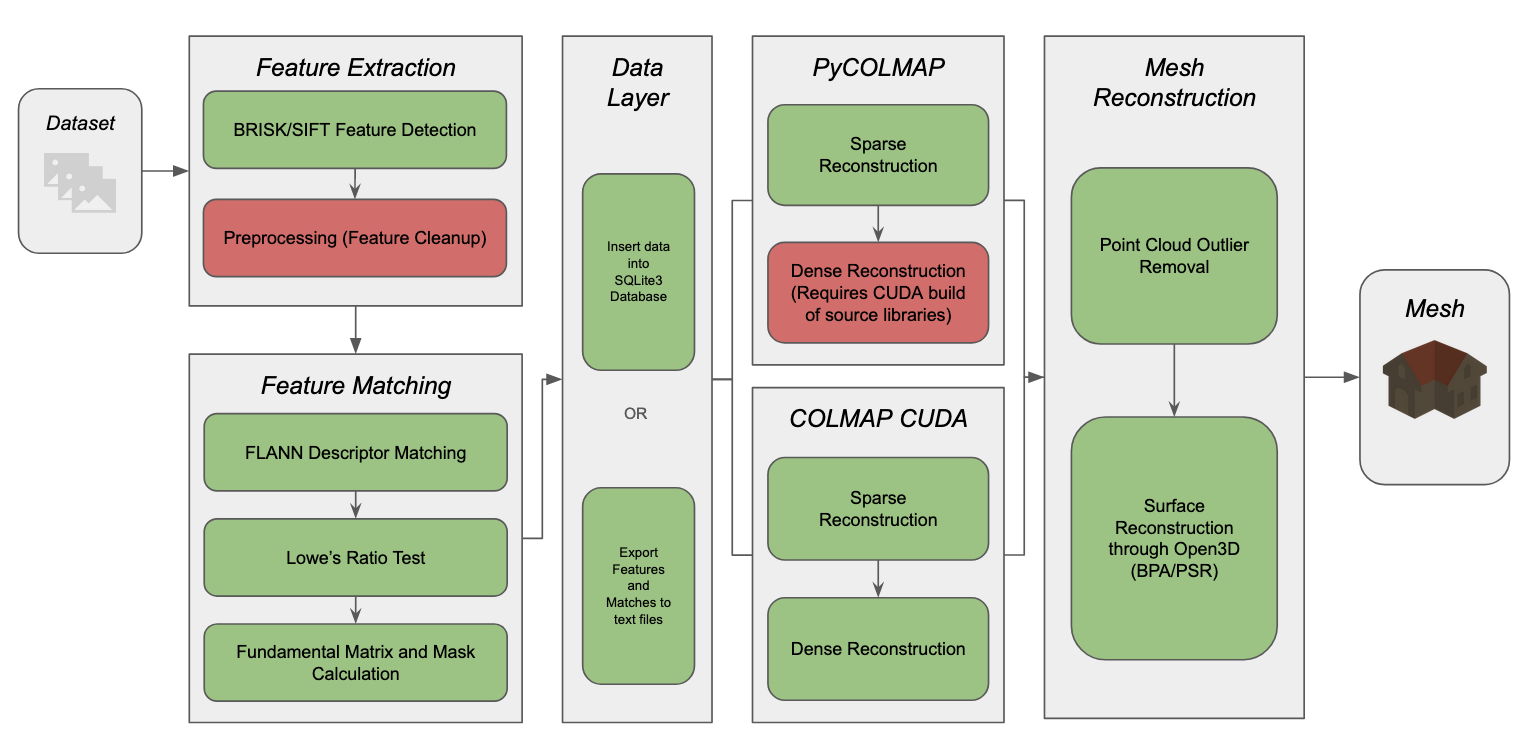
\includegraphics[width=.4\textwidth]{figures/pipeline.png} }}
    \caption{Pipeline/Project Workflow}
    \label{fig:pipeline}
  \end{figure}
\subsection{SFM-MVS}
SFM algorithms generally consist of the following steps: 
feature extraction, feature matching, triangulation, and bundle adjustment. 
\\
Traditionally, feature extraction in SFM algorithms use Lowe's 
SIFT approach for both feature detection and description \cite{sift}.
Detection in SIFT involves a Gaussian pyramid-like structure of octaves 
for scale space representation. Each octave of scale space contains a 
set of Gaussian convolved images separated by a scale factor, 
and each octave uses a down-sampled image relative to the previous 
octave. The extrema (within a given window) of a difference-of-Gaussian 
(DoG) (Figure \ref{fig:sift_scale_space}) function applied to adjacent Gaussian images within 
octaves is used to detect stable key points in scale space. 
Mathematically, the scale space is defined as a function 
$L(x,y,\sigma)$, produced from a variable-scale Gaussian,
$G(x,y,\sigma)$ and the input image $I(x,y)$ \cite{sift}:
\[
    L(x,y,\sigma) = G(x,y,\sigma) * I(x,y)
\] where $*$ is the convolution operation. The DoG function takes the form:
\begin{flalign*}
    D(x,y,\sigma) &= (G(x,y,k\sigma) - G(x,y,\sigma)) * I(x,y) \\
    &= L(x,y,k\sigma) - L(x,y,\sigma)
\end{flalign*}
with some constant multiplicative scale factor $k$. 
\begin{figure}[ht!]
    \centering
    {{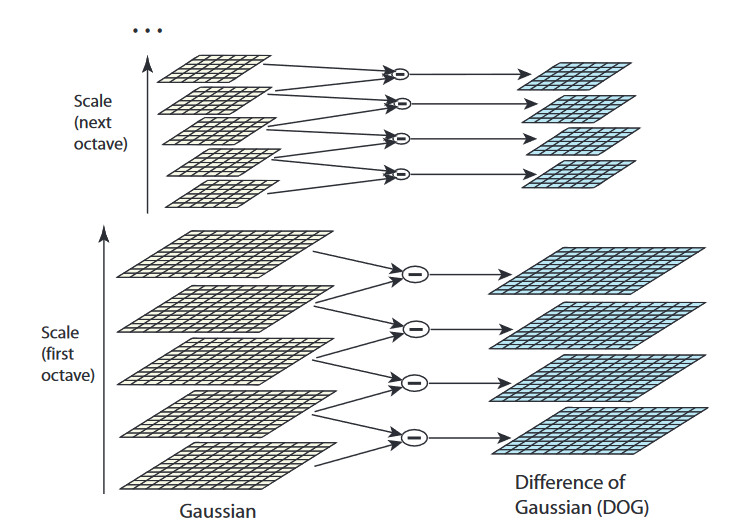
\includegraphics[width=.4\textwidth]{figures/sift_scale_space.png} }}
    \caption{Difference of Gaussians and Sift Scale Space\\Source: Adapted from \cite{sift}}
    \label{fig:sift_scale_space}
\end{figure}
DoG approximates the normalized Laplacian of Gaussian \cite{lindeberg}
, whose local extrema was shown to correspond to stable key points/blobs. 
SIFT descriptors \cite{sift} take the gradient directions over a 
spatial region around feature points. A histogram of these gradient 
directions (orientations) is normalized and invariant against rotation, 
scale, and brightness. The descriptors are stored as a 128-dimensional 
vector containing these histogram values corresponding to the gradient 
magnitudes and are known for their distinctiveness. BRISK feature detection
\cite{brisk} builds on a computationally optimized version of 
FAST 9-16 adapted for scale invariance via a simplified representation of 
scale space (compared to SIFT \cite{sift}). Due to the simplified scale 
space representation and use of a computationally efficient FAST 9-16 
detection algorithm, BRISK is considerably faster than SIFT while still 
detecting high quality key points. The set of detected points with BRISK is 
similar to many SIFT detected points. Additionally, since both approaches 
revolve around scale, rotation, and illuminance invariance, and since description 
is independent of detection, SIFT descriptors can be easily applied to BRISK key 
points. For the purposes of this project, we rely on OpenCV's 
implementation of both SIFT \cite{siftcv} and BRISK \cite{briskcv}.
Feature matching in SFM (with SIFT descriptors) is done by identifying 
a nearest neighbor (based on L2 distance) between descriptors in 2 views \cite{sift}.
This is efficiently approximated through \cite{fnn}.\\
Lowe's ratio test \cite{sift} compares the distance measures of 
the 2 nearest neighbors and rejects matches where the ratio between the 
distances from these neighbors is greater than or equal to some value $l$ (ie.
$d_1 \ge l \cdot d_2)$, eliminating false matches. \cite{usac}'s 
MAGSAC++ \cite{magsac}, an improved version of RANSAC, further 
refines these matches by finding inliers during a fundamental 
matrix estimation between randomly sampled matches. 
Two view geometry estimation, triangulation and bundle adjustment, 
as well as multiview stereo, are handled through COLMAP \cite{colmap}
\cite{schoenberger2016sfm} \cite{schoenberger2016mvs}, resulting in sparse 
and dense point cloud reconstructions (with estimated surface normals).

% \subsubsection{Image Capturing}
% Image capturing techniques for SFM

\subsection{Feature Preprocessing}
During feature extraction, further processing can be 
done to isolate key points on objects. We apply a combination of 
image filtering, blurring, and canny edge detection to build a binary mask
(show in Figure \ref{fig:mask}) covering the object of interest. 
\begin{figure}[ht!]
    \centering
    \subfloat[Initial Image]{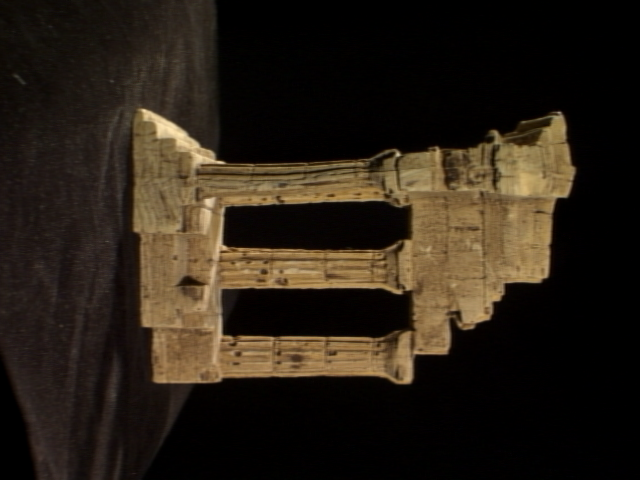
\includegraphics[width=.2\textwidth]{figures/temple.png}}
    \
    \subfloat[Binary mask]{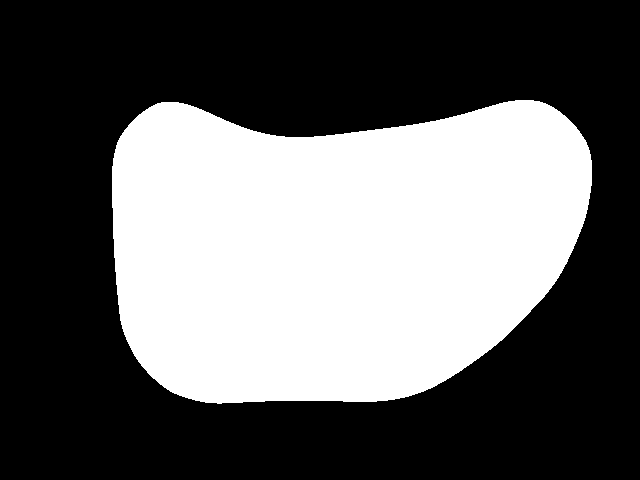
\includegraphics[width=.2\textwidth]{figures/temple_mask.png}}
    \caption{Binary Mask}
    \label{fig:mask}
\end{figure}
This mask is used to discard key points which are determined to be background noise.
Preparation for canny edge detection involves noise reduction through a gaussian blur
for effective detection \cite{ced}. Though OpenCV's implementation \cite{ced_ocv}
applies a $5\times 5$ Gaussian kernel, further reduction is often necessary.
Additionally, we apply a DoG (shown in Figure \ref{fig:DoG_ppc}) based approach to accentuate edges and blobs 
for lower texture objects and noisier datasets. 
\begin{figure}[ht!]
    \centering
    \subfloat[Gaussian $g_0$]{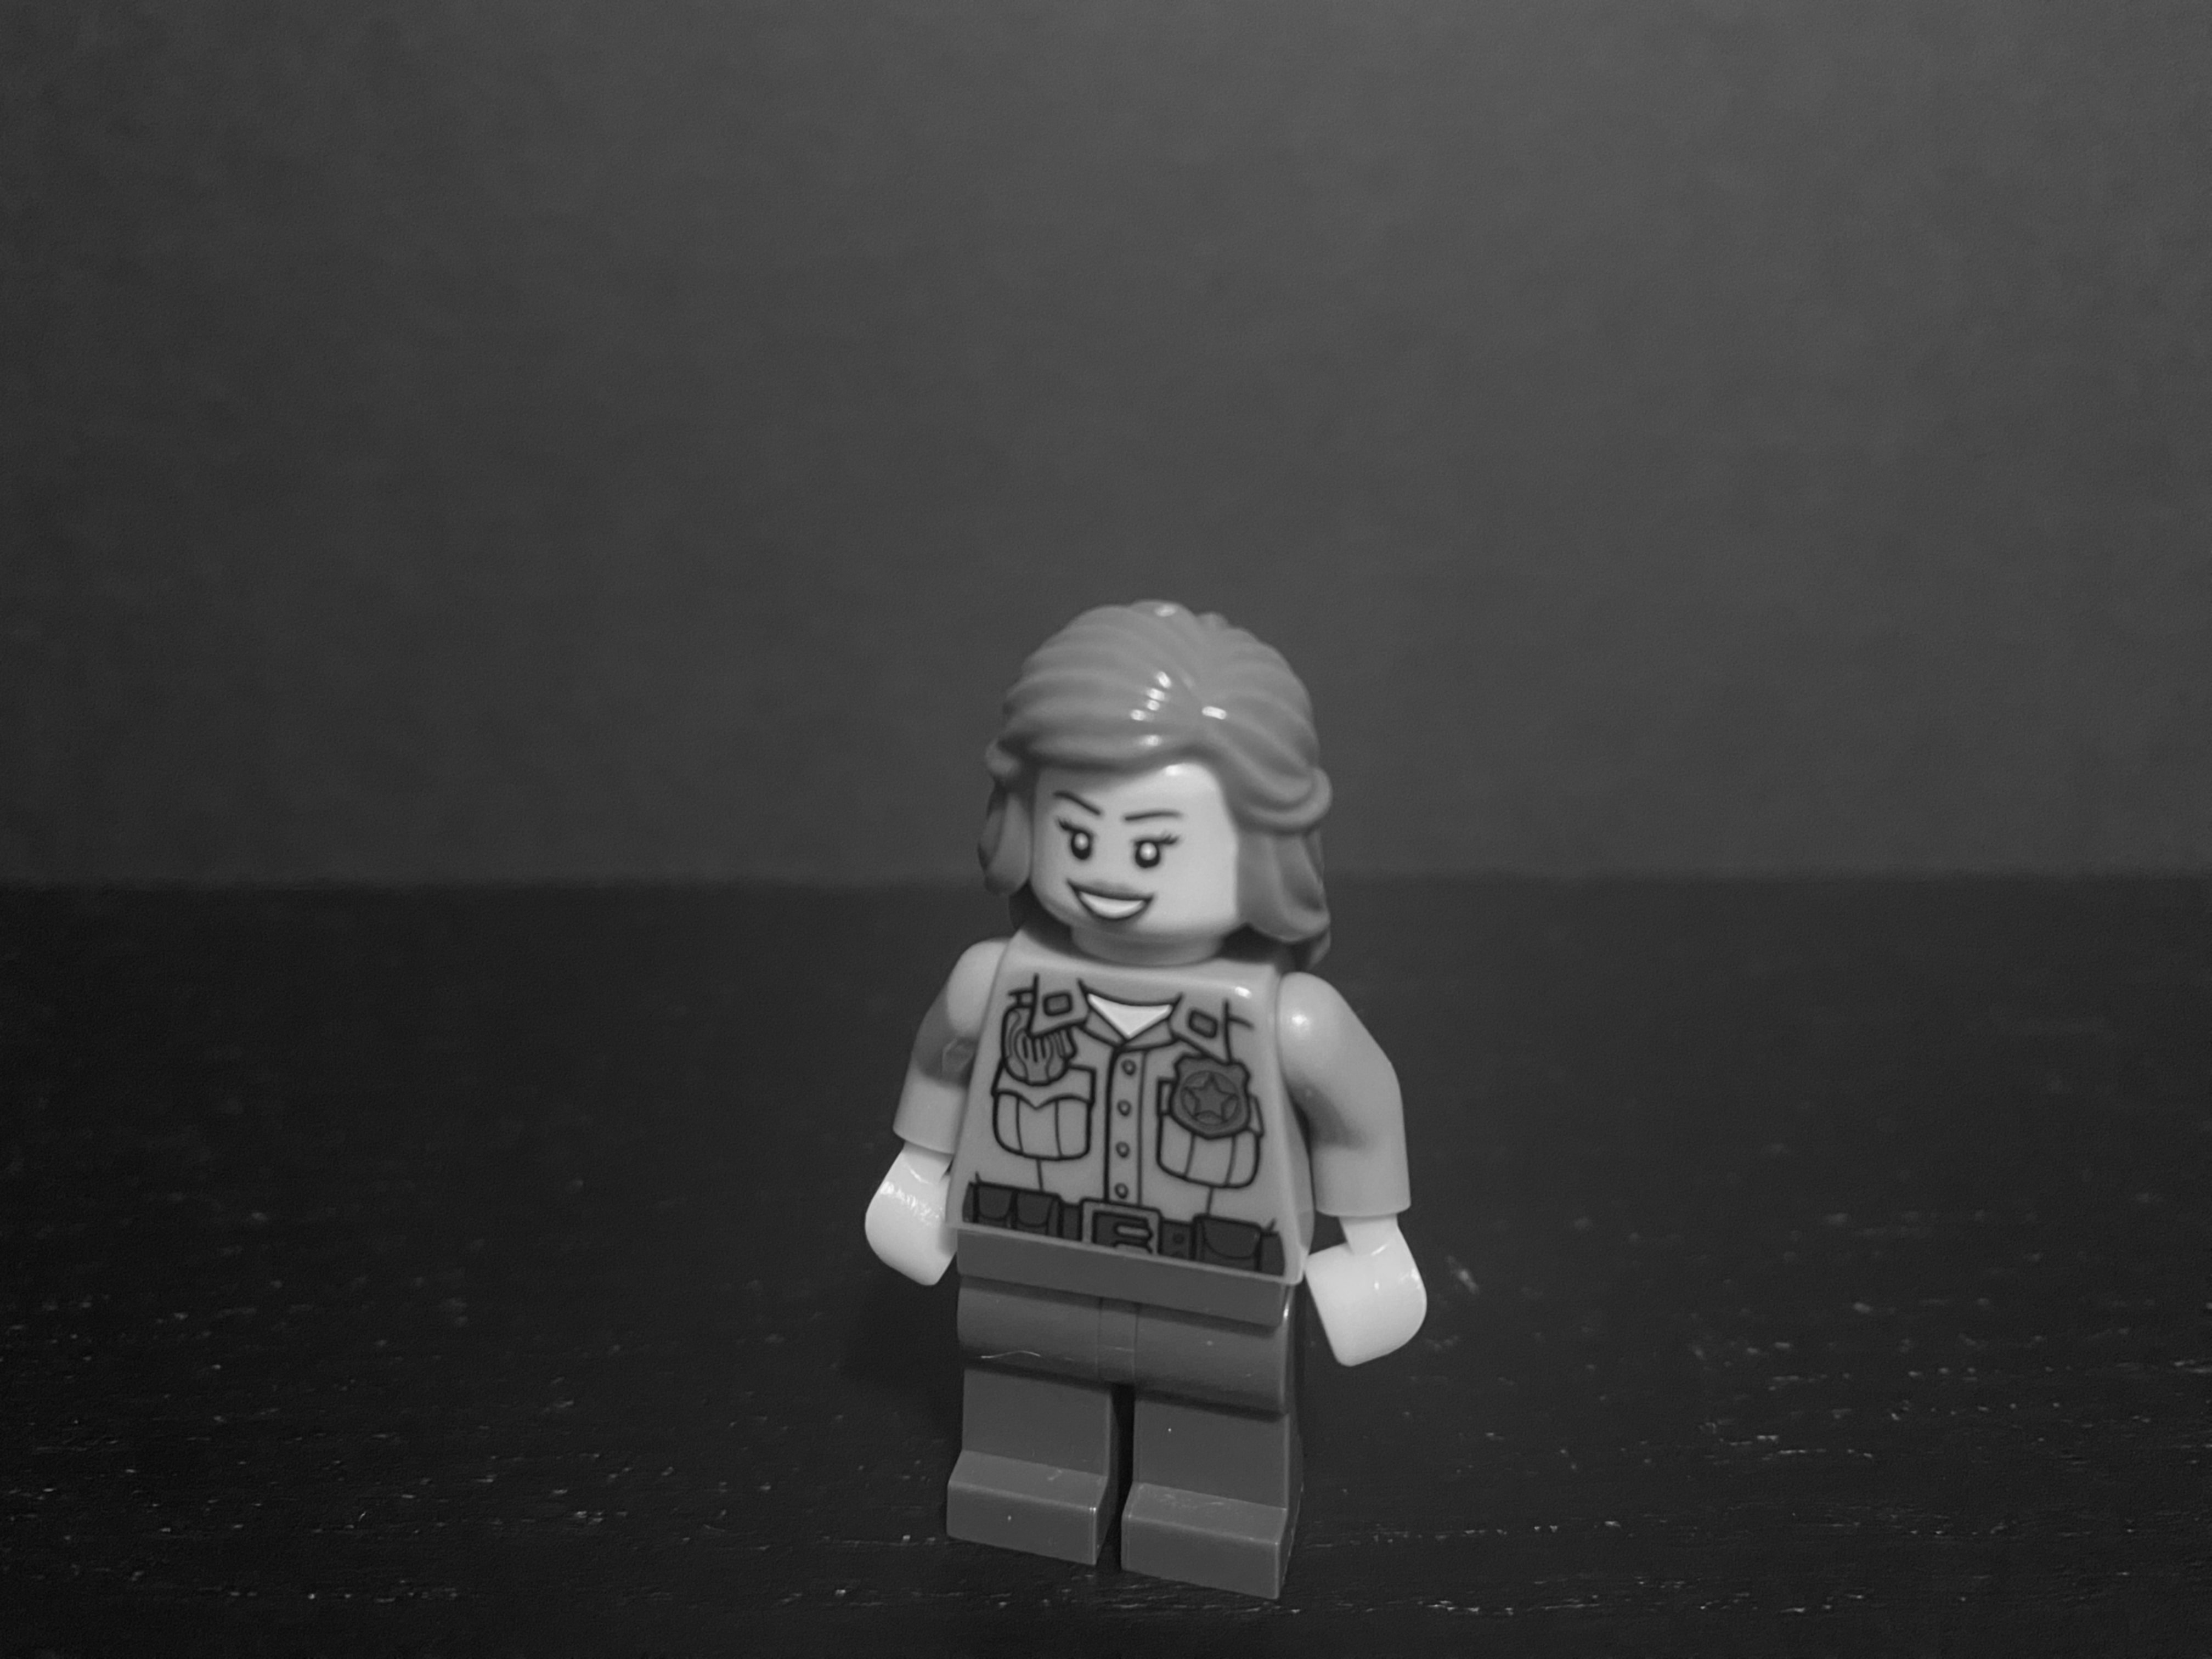
\includegraphics[width=.2\textwidth]{figures/dog/g0.png}}
    \
    \subfloat[Scaled Gaussian $g_1$]{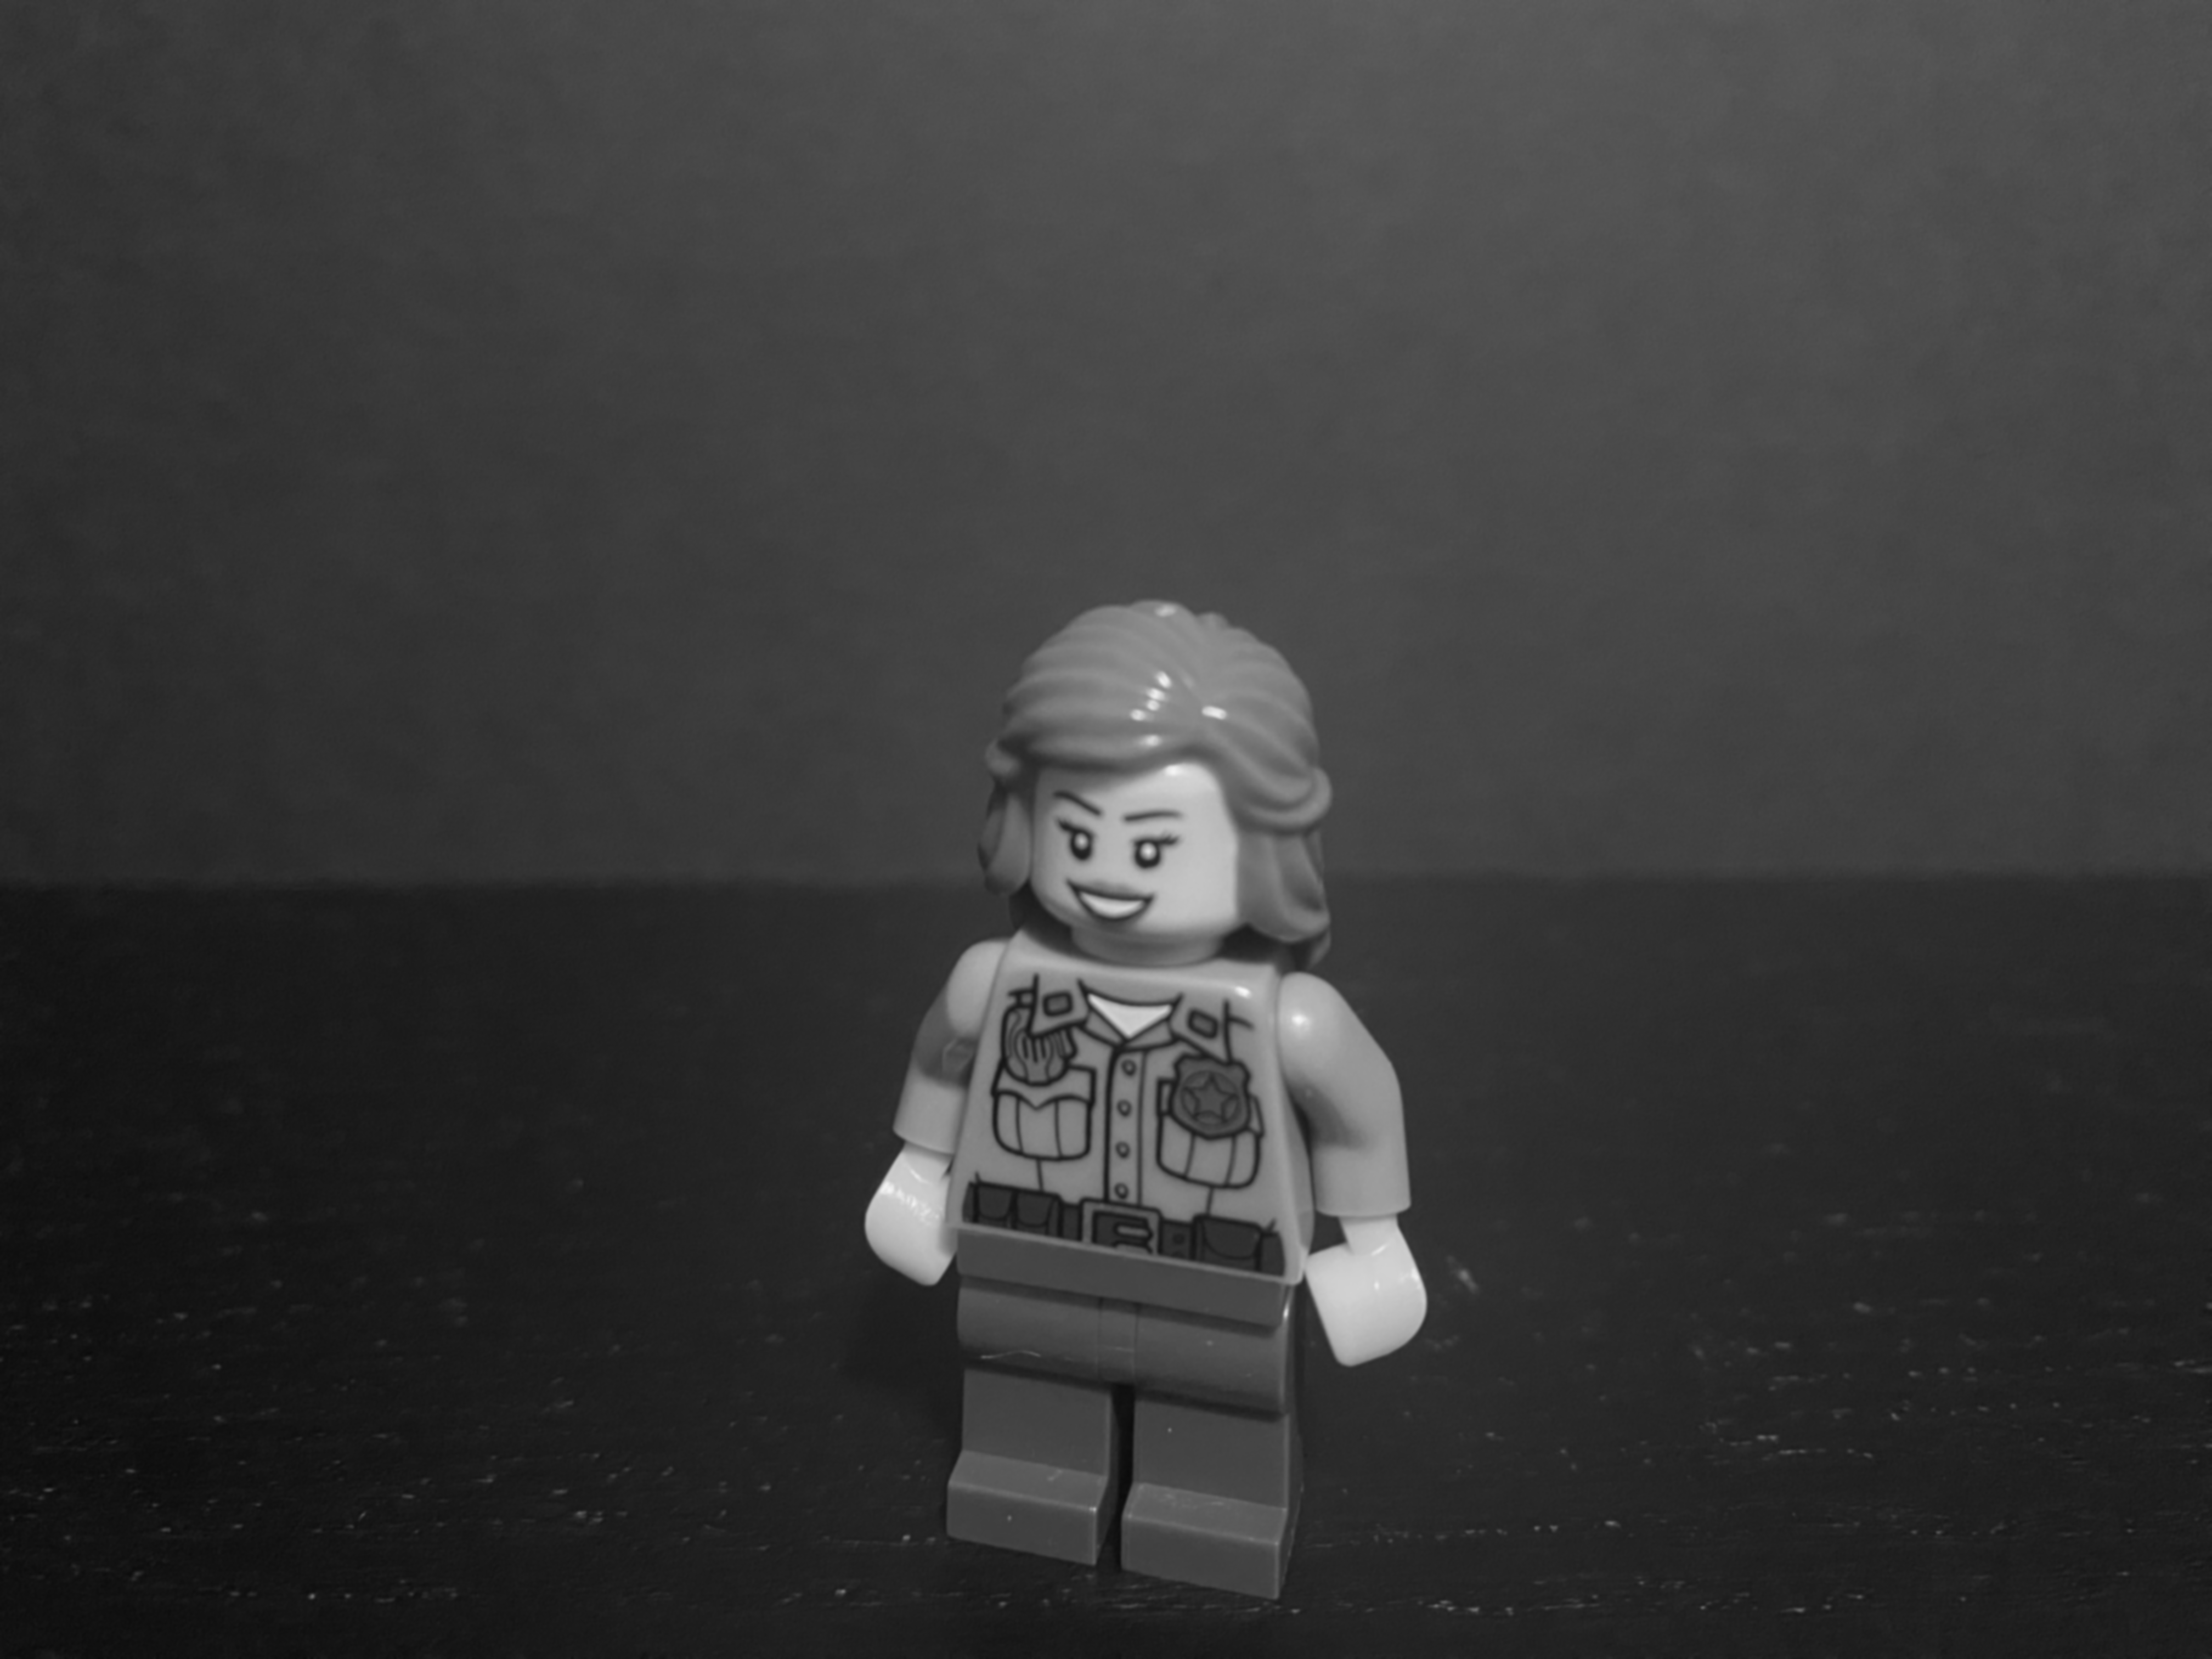
\includegraphics[width=.2\textwidth]{figures/dog/g1.png}}
    \\
    \subfloat[DoG ($g_1-g_0$)]{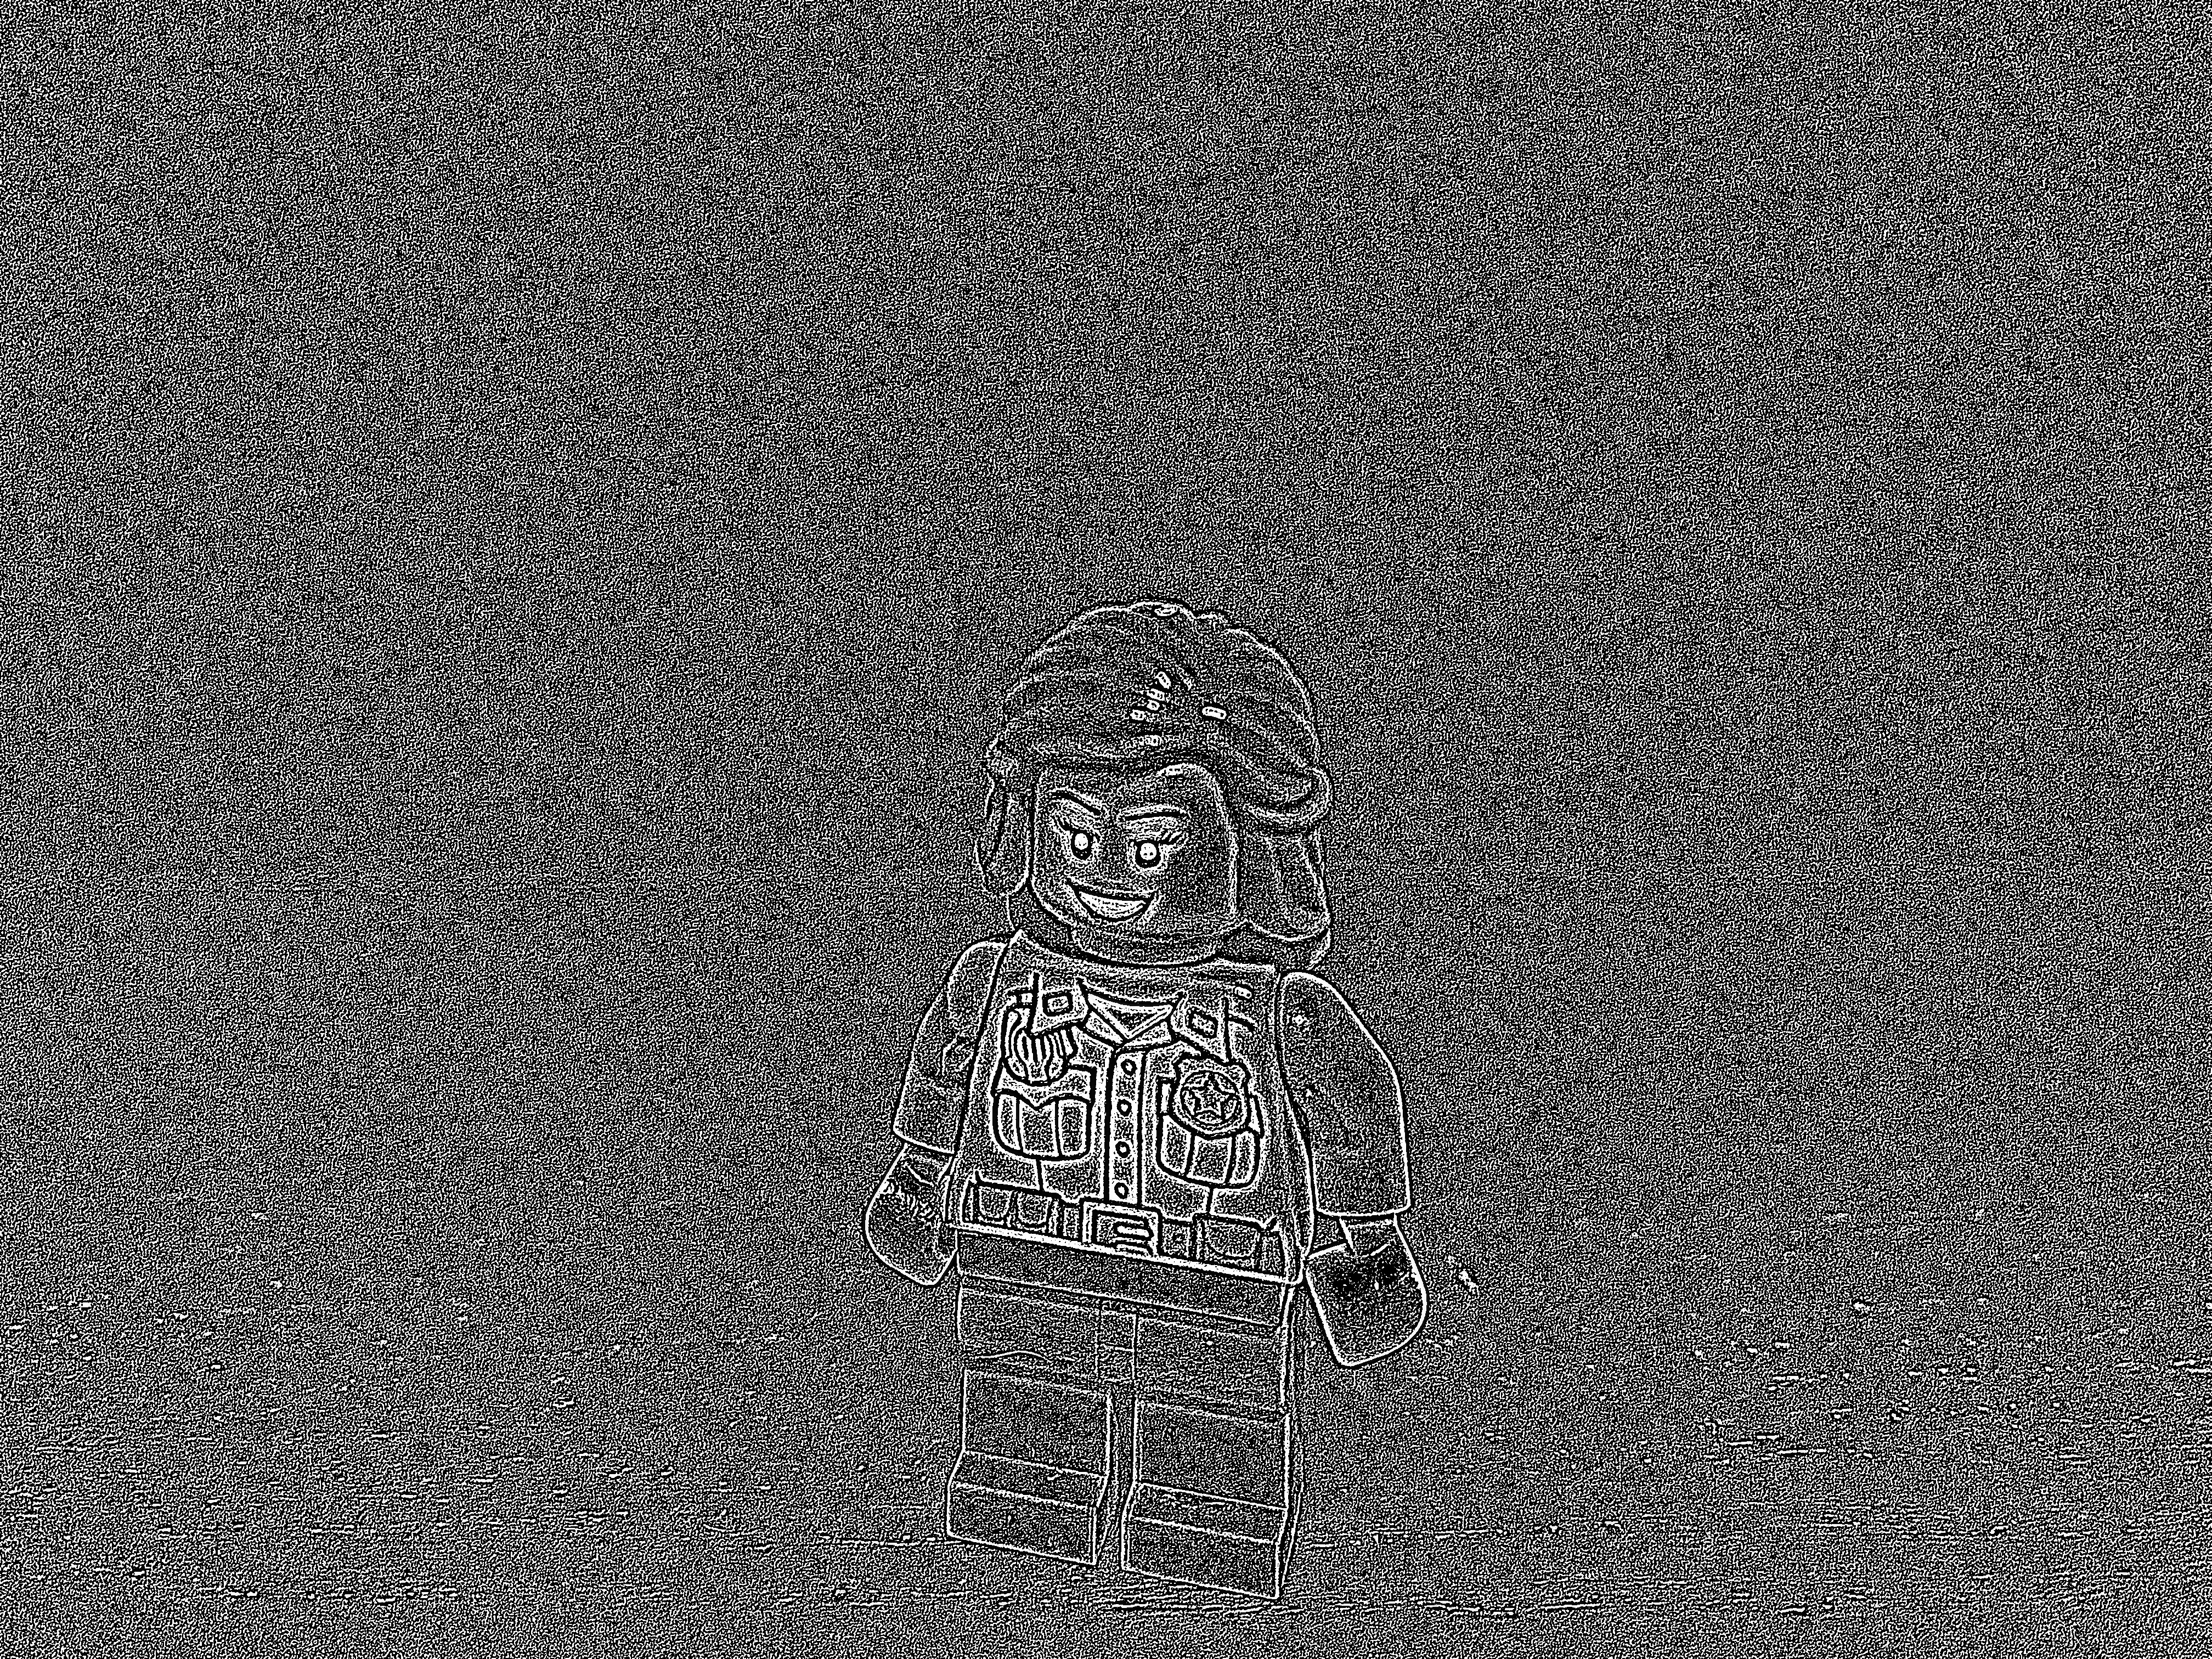
\includegraphics[width=.2\textwidth]{figures/dog/dog.png}} \
    \subfloat[Blurred DoG (smoothen noise; prep. for edge detection)]{\includegraphics[width=.2\textwidth]{figures/dog/bdog.png}}
    \\
    \subfloat[Mask (No DoG)]{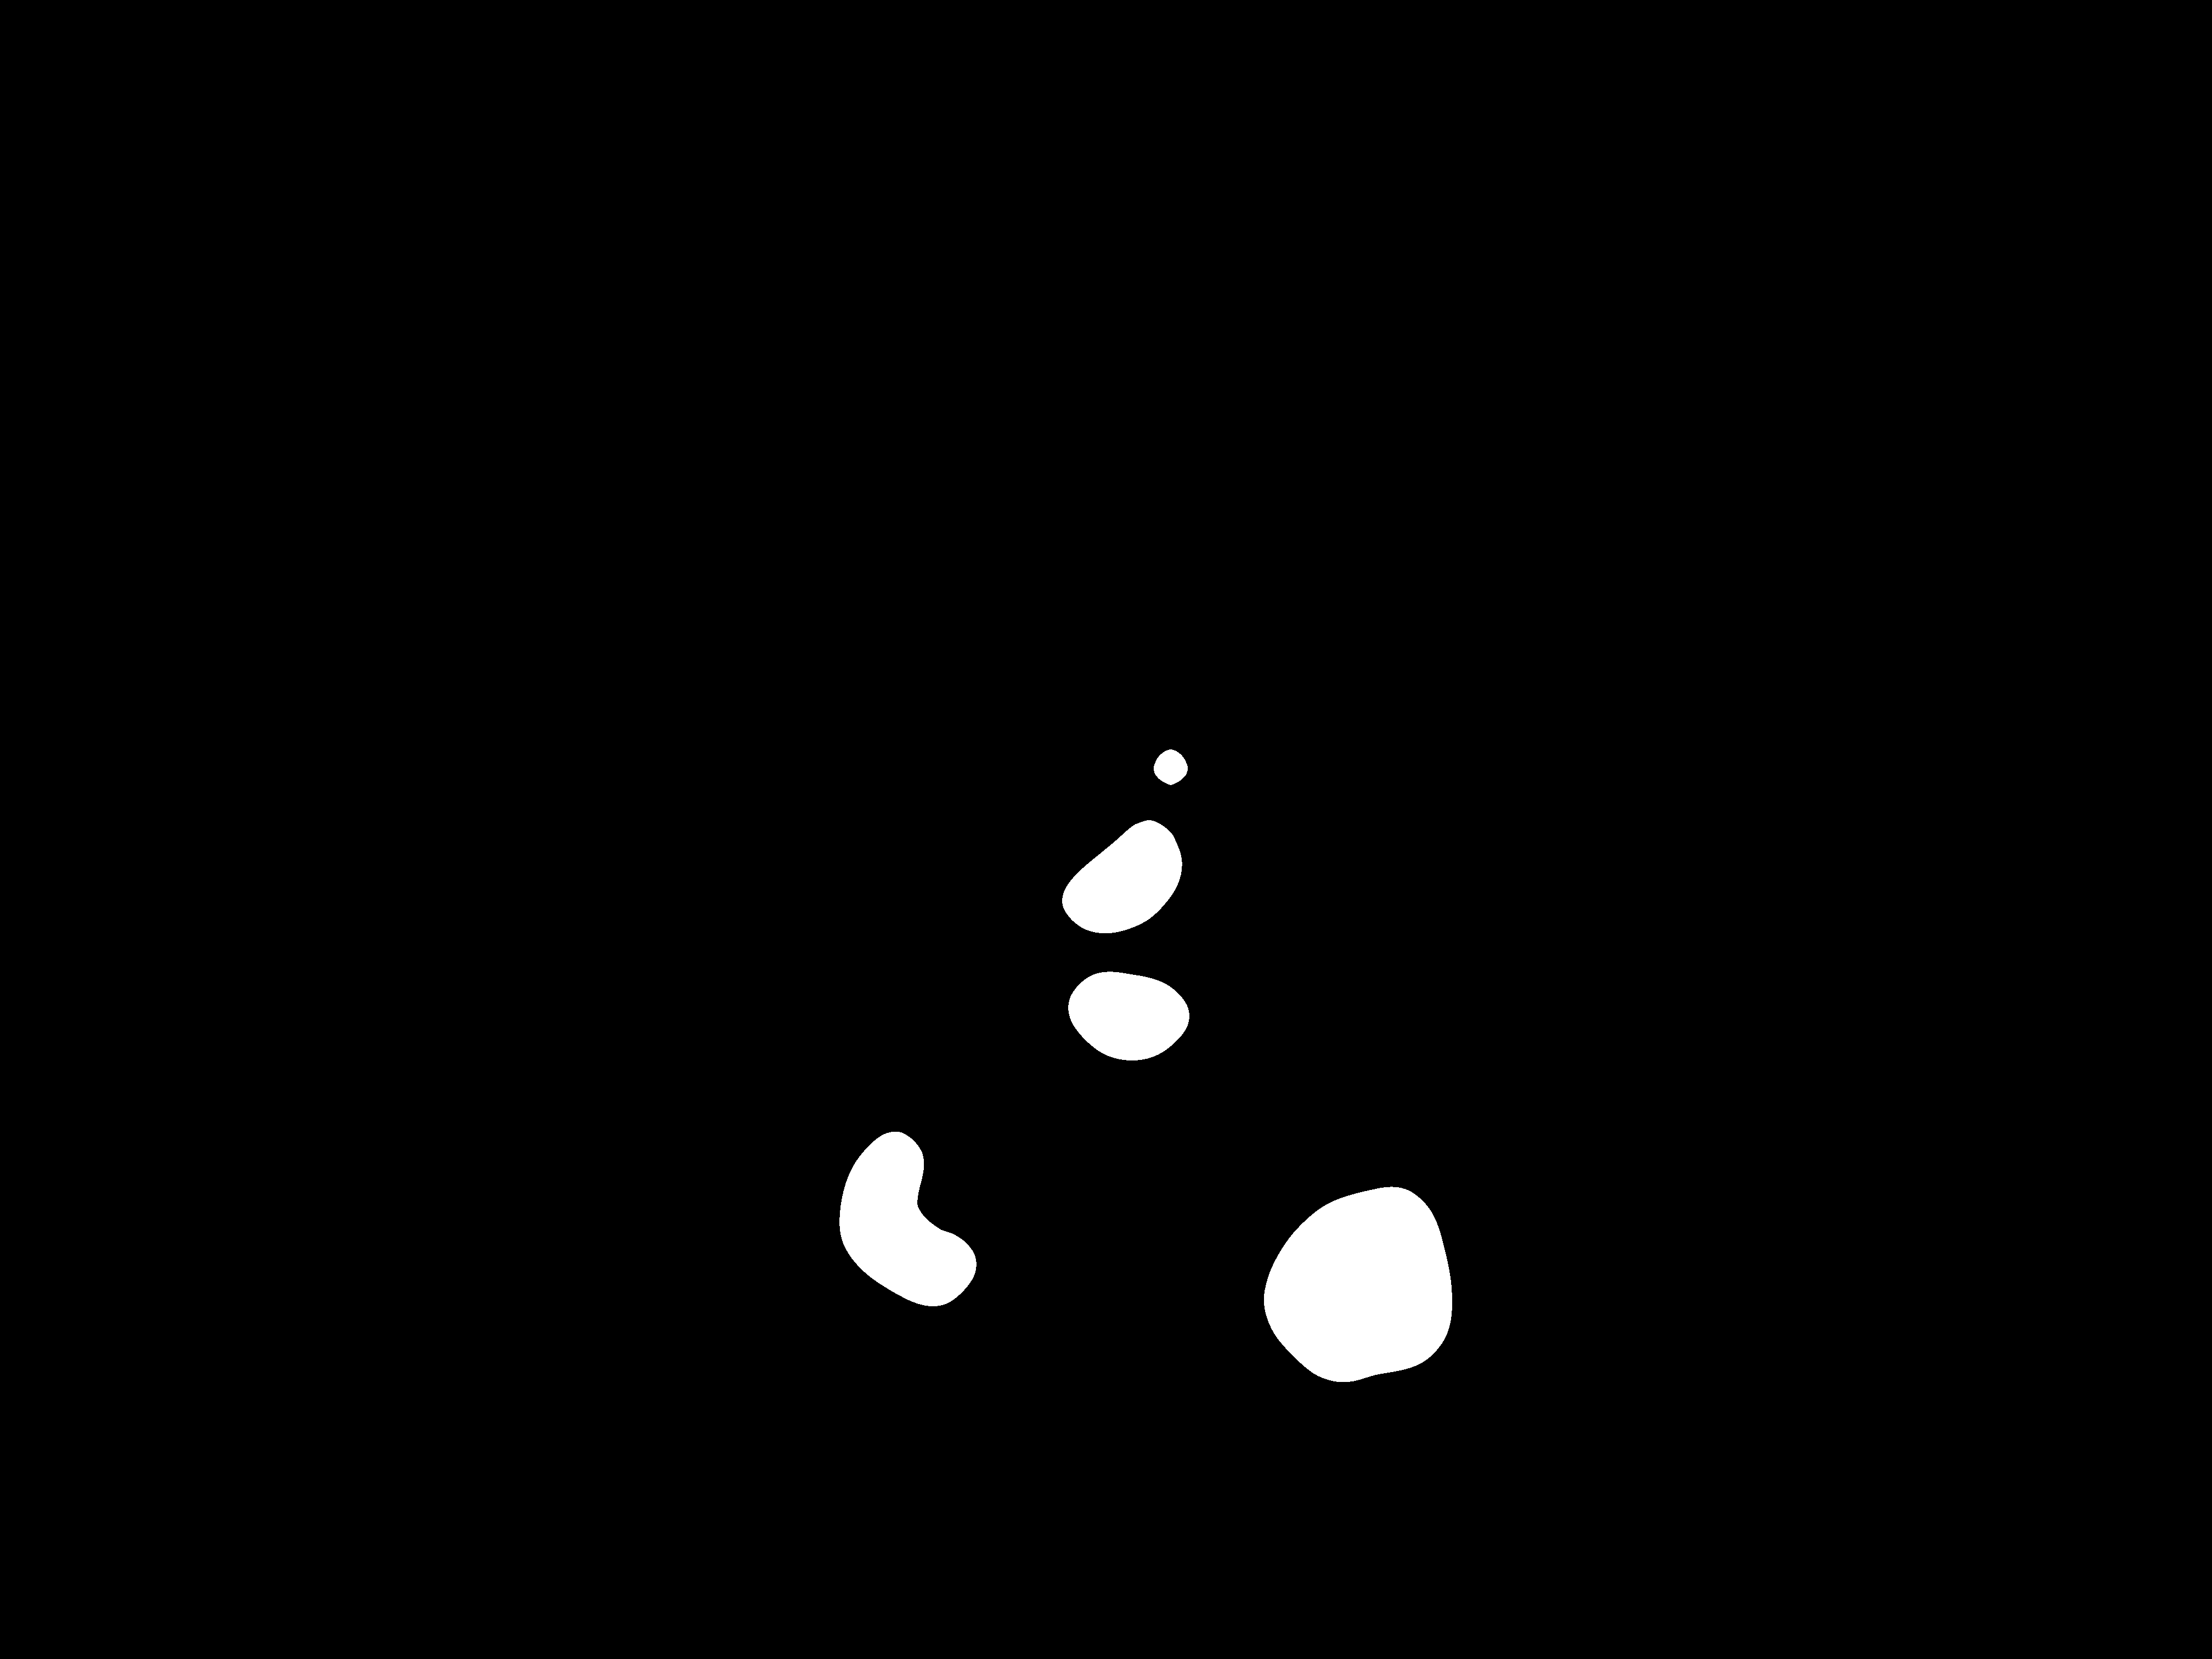
\includegraphics[width=.2\textwidth]{figures/dog/bad_mask.png}}
    \
    \subfloat[Mask (DoG)]{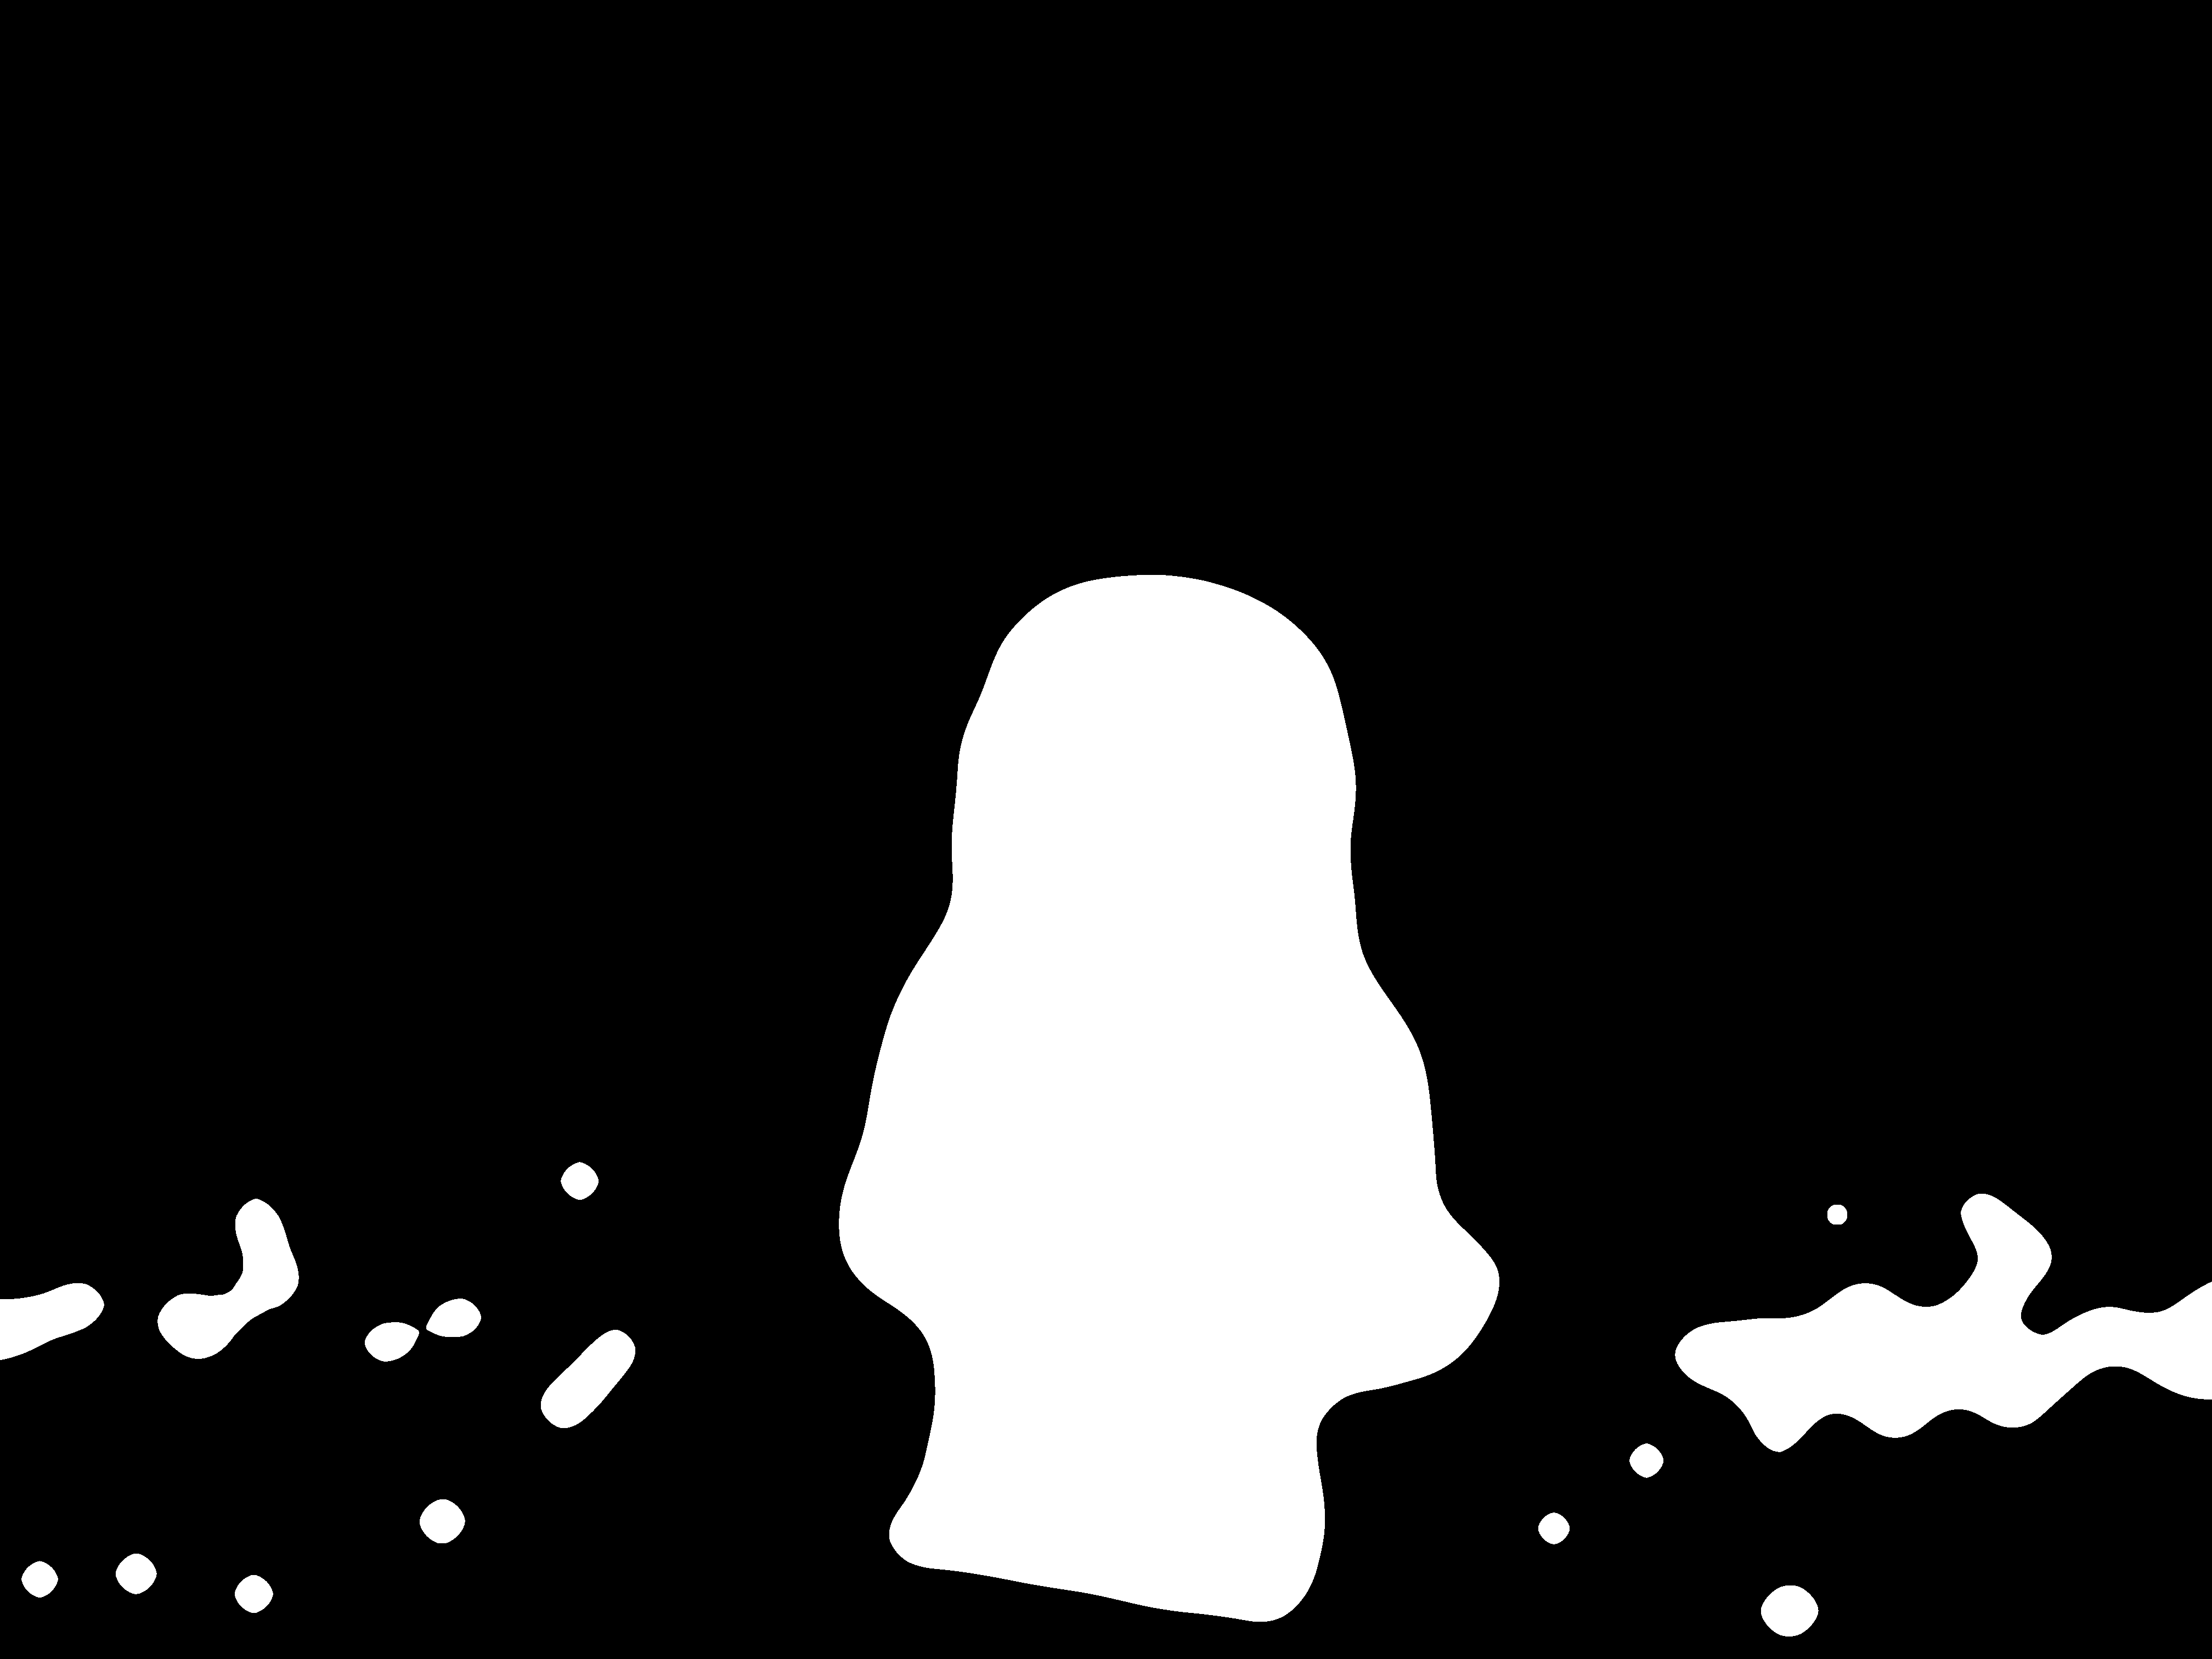
\includegraphics[width=.2\textwidth]{figures/dog/mask.png}}
    \caption{Difference of Gaussian based preprocessing approach. ($\sigma$-scale factor $k=2$)
    Inspired by \cite{sift}.}
    \label{fig:DoG_ppc}
\end{figure}
Sobel filters applied in the horizontal and vertical directions 
allow us to obtain edge gradients and directions \cite{ced_ocv} as follows:
\[
    G = \sqrt{G_x^2 + G_y^2}, \ \ \ \theta = \arctan \left( \dfrac{G_y}{G_x} \right)
\] where $G$ is the edge gradient and $\theta$ is the edge direction.
\\
Non-maximum suppression removes unwanted pixels that may not be part of an edge \cite{}.
Hystersis thresholding determines edge criterion via a user defined 
lower-upper bound $(l,u)$:
\begin{enumerate}[i]
    \item $G > u$ $\to$ edge
    \item $G < l$ $\to$ not an edge
    \item $G \in [l,u]$ $\to$ classified based on connectivity to edge pixels
\end{enumerate}
We use the edge image, $E(x,y)$, to build a mask by:
\begin{enumerate}[1.]
    \item Convolving a Gaussian kernel on $E$
    \item Binary thresholding is applied to the convolved image (forming the initial mask $M$)
    \item Apply two median blur filters to $M$
\end{enumerate}
We can apply our mask to the source frame and exclude key points that
are irrelevant to the image. Though this does not directly affect the dense point cloud
reconstruction from MVS, it can decrease matches from background noise, thus 
improving match performance and the accuracy of two view geometry. A general 
outline of our feature preprocessing approach is shown in Figure \ref{fig:ppc_pipe}
and an example is how in Figure \ref{fig:ppc}
\begin{figure}[ht!]
    \centering
    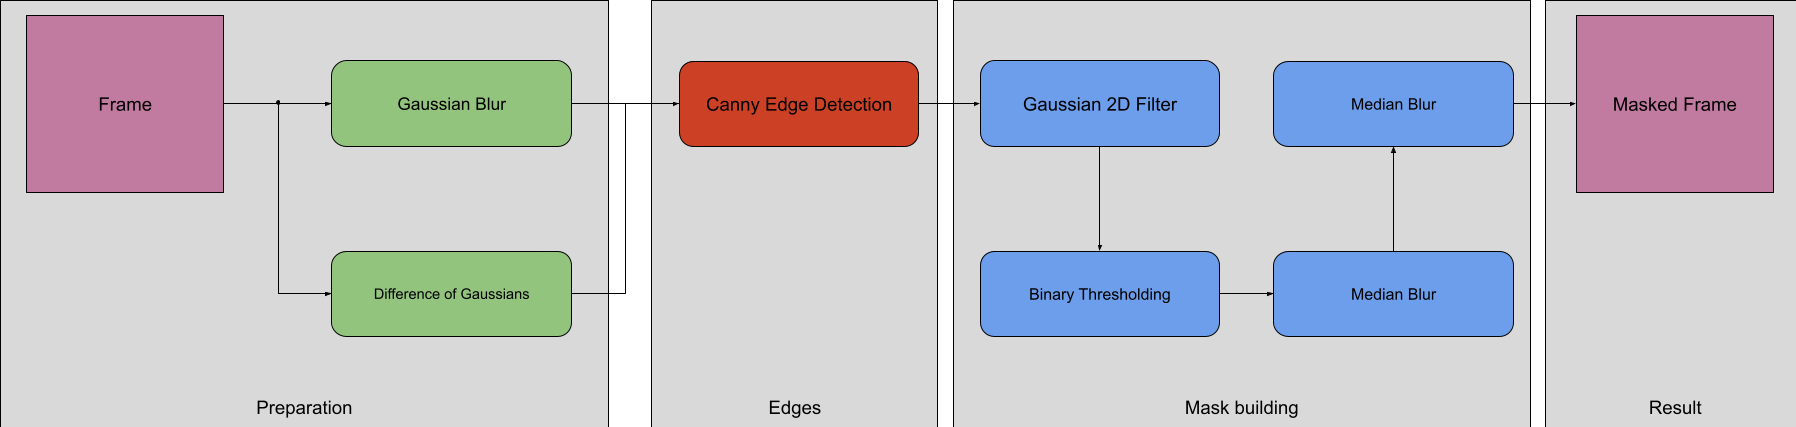
\includegraphics[width=.4\textwidth]{figures/preproc pipeline.png}
    \caption{Feature preprocessing pipeline}
    \label{fig:ppc_pipe}
\end{figure}
\begin{figure}[ht!]
    \centering
    \subfloat[Source Image]{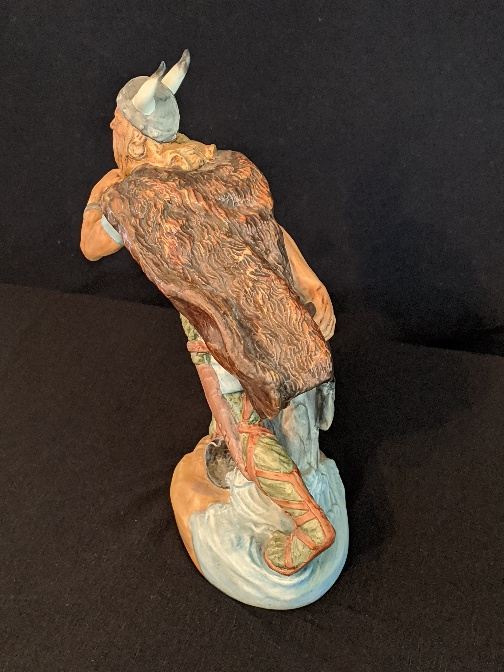
\includegraphics[width=.2\textwidth]{figures/ppc/src.png}}
    \
    \subfloat[BRISK keypoints]{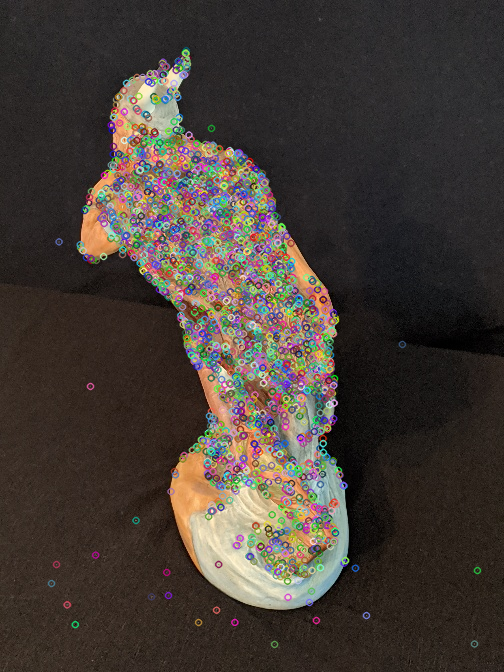
\includegraphics[width=.2\textwidth]{figures/ppc/kp.png}}
    \\
    \subfloat[Edge]{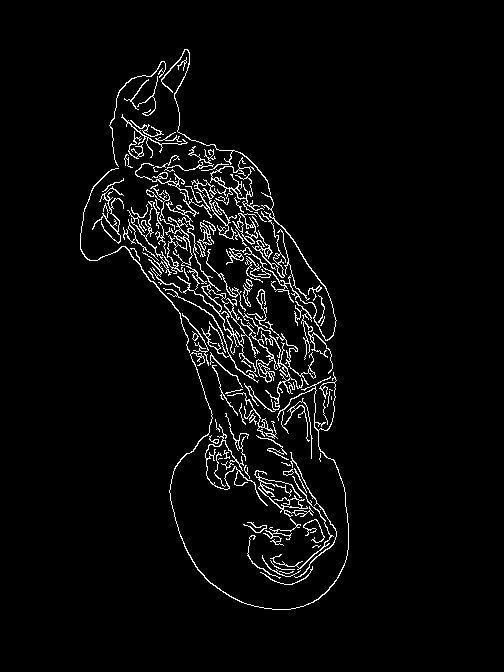
\includegraphics[width=.13\textwidth]{figures/ppc/edge.png}}
    \
    \subfloat[Mask]{
\includegraphics[width=.13\textwidth]{figures/ppc/mask.png}}
    \
    \subfloat[Masked image]{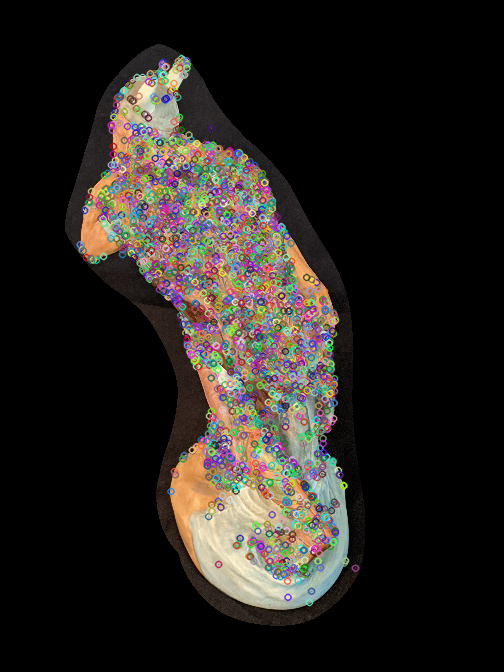
\includegraphics[width=.13\textwidth]{figures/ppc/mkp.png}}
    \caption{Feature preprocessing example}
    \label{fig:ppc}
\end{figure}

\subsection{Point Cloud Processing}
This project uses Open3D's implementation of the Ball-Pivot Algorithm (BPA) \cite{bpa}
\cite{sr_o3d} and Poisson Surface Reconstruction (PSR) \cite{psr}\cite{sr_o3d}, 
two widely used mesh reconstruction techniques. 
BPA involves a “ball” with a user-defined radius, $r$, 
which pivots along a manifold surface of the 3D object.
Triangles are formed when the ball touches 3 points 
without “falling through”, eventually leading to a triangle mesh 
once all points are considered \cite{bpa}. This process can be 
repeated with various different radii to improve accuracy. 
An implementation trick we discovered with radii tuning was 
defining them as an array of scaled average neighbor distances. 
This approach often gave the best results with respect to BPA.
PSR \cite{psr} formalizes surface reconstruction as a 
poisson problem and creates very smooth surfaces that 
robustly approximate noisy data using a point cloud, 
its normals, and an octree of a user specified depth. 
However, PSR assumes the point cloud represents an object 
rather than the environment surrounding it, as such its 
robustness to noise is limited when background points are 
introduced. Additionally, BPA \cite{bpa} is generally 
not as robust as PSR for noise in an object point cloud, 
however it handles background noise well 
(given enough separation between points). 
To alleviate the effect of noise, we use 
Open3D's radial and statistical point cloud outlier removal 
algorithms to automate background noise removal \cite{pcr},
improving overall mesh quality for both approaches. 

% \section{Results}

% \section{Conclusions}


% \section{}





% \section{Conclusion}
% The conclusion goes here.




% conference papers do not normally have an appendix



% use section* for acknowledgment
% \ifCLASSOPTIONcompsoc
%   % The Computer Society usually uses the plural form
%   \section*{Acknowledgments}
% \else
%   % regular IEEE prefers the singular form
%   \section*{Acknowledgment}
% \fi


% The authors would like to thank...





% trigger a \newpage just before the given reference
% number - used to balance the columns on the last page
% adjust value as needed - may need to be readjusted if
% the document is modified later
%\IEEEtriggeratref{8}
% The "triggered" command can be changed if desired:
%\IEEEtriggercmd{\enlargethispage{-5in}}

% references section

% can use a bibliography generated by BibTeX as a .bbl file
% BibTeX documentation can be easily obtained at:
% http://mirror.ctan.org/biblio/bibtex/contrib/doc/
% The IEEEtran BibTeX style support page is at:
% http://www.michaelshell.org/tex/ieeetran/bibtex/
%\bibliographystyle{IEEEtran}
% argument is your BibTeX string definitions and bibliography database(s)
%\bibliography{IEEEabrv,../bib/paper}
%
% <OR> manually copy in the resultant .bbl file
% set second argument of \begin to the number of references
% (used to reserve space for the reference number labels box)
% \begin{thebibliography}{1}

% \bibitem{IEEEhowto:kopka}
% H.~Kopka and P.~W. Daly, \emph{A Guide to \LaTeX}, 3rd~ed.\hskip 1em plus
%   0.5em minus 0.4em\relax Harlow, England: Addison-Wesley, 1999.

% \end{thebibliography}

\bibliographystyle{IEEEtran}
\bibliography{References}


% that's all folks
\end{document}


